

\begin{frame}{\ft{Filtering Photos}}
\section{E-Commerce Slide 6}
\doubleFrame{Another feature which may be conveniently 
implemented in A3R-style photo viewers is a filtering 
option, which --- given a collection of pictures 
classified into several groups --- allows users 
to show or hide photos based on the group they belong to (note the check-box buttons on the group listing).}

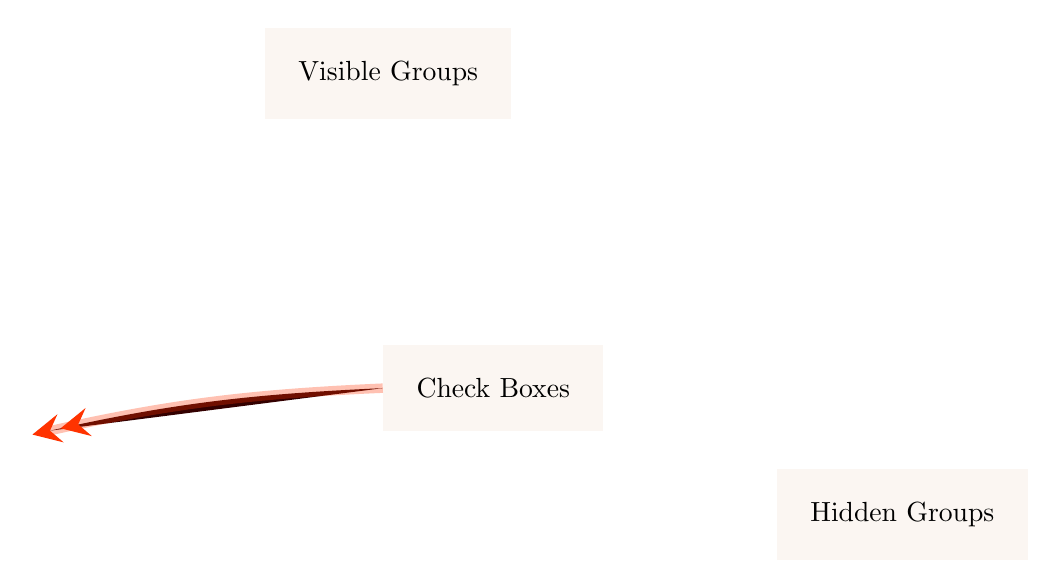
\begin{tikzpicture}

\nodeincludegraphicsTRRS{1}{4cm}{0.05cm}{3cm}{1.35cm}{screenshots/ss-ph4.png}


\node [anchor=west,fill=brown!8!white,inner sep=12, 
opacity=0.88, text opacity=1] (note) at (4.5,8.2) {\hc{Visible Groups}};


\ann{BlueGreen}{1}{.8mm}{grammarArrowColor}{0.5}{3.61,5.5}{2.4}{.6}{0.7}
%\ann{BlueGreen!30!red}{1}{.8mm}{blue!50!orange}{0.5}{3.61,5.5}{2.4}{.6}{0.7}

%{BlueGreen}{0.3}{1mm}{grammarArrowColor}{0.5}

\colorarr{>=latex, ->}{fcBoxColor!60!black}
{0.8}{blGreen!30!red}{2}{1mm}{note.south}{6, 5.9}



\node [anchor=west,fill=brown!8!white,inner sep=12, 
opacity=0.88, text opacity=1] (cb) at (6,4.2) {\hc{Check Boxes}};

\draw[>=stealth, ->>,bend right=5, 
draw=orange!40!red,% rgb{0.5,0.1,0.4}, 
draw opacity=0.3,
fill=red!20!black, fill opacity=1, 
line width=1.2mm
] (cb.west) to (1.55, 3.61);


\node [anchor=west,fill=brown!8!white,inner sep=12, 
opacity=0.88, text opacity=1] (note) at (11,2.6) {\hc{Hidden Groups}};


\ann{BlueGreen!30!red}{1}{.8mm}{blue!50!orange}{0.5}{3.61,1.7}{2.4}{.6}{0.7}

\colorarr{>=latex, ->}{fcBoxColor!20!black}
{0.8}{darkRed!70!blue}{2}{1mm}{note.west}{6, 1.9}


%\node [anchor=west,fill=brown!8!white,inner sep=12, 
%opacity=0.88, text opacity=1] (note) at (6.7,9.7) {\hc{Not Yet Viewed (horizontal color band)}};

%\ann{BlueGreen!30!red}{1}{.8mm}{blue!50!orange}{0.5}{7.6, 7.3}{.73}{.35}{0.7}

%\colorarr{>=latex, ->}{fcBoxColor!20!black}
%{0.8}{darkRed!70!blue}{2}{1mm}{note.south}{8.2, 7.25}



%\node [anchor=west,fill=brown!8!white,inner sep=12, 
%opacity=0.88, text opacity=1] (note) at (5,1.89) {\hc{Current Photo (viewed for the second time)}};

%\colorarr{>=latex, ->}{fcBoxColor!60!black}
%{0.8}{blGreen!30!red}{1}{1mm}{note.north west}{4.35, 4.75}


\end{tikzpicture}


\end{frame}

